\documentclass[11pt, oneside]{article}
\usepackage[margin=1in]{geometry}
\geometry{letterpaper}
\usepackage{booktabs}
\usepackage{hyperref}
\usepackage{enumitem}
\setlist{itemsep=1.5pt, topsep=2pt, parsep=0pt, partopsep=0pt}
\setlength{\parskip}{1.5pt}
\setlength{\floatsep}{6pt plus 2pt minus 2pt}
\setlength{\textfloatsep}{8pt plus 2pt minus 2pt}
\setlength{\intextsep}{6pt plus 2pt minus 2pt}
\usepackage{float}
\usepackage{caption}
\usepackage{subcaption}
\usepackage[numbers]{natbib}
\usepackage{graphicx}
\usepackage{amssymb}
\usepackage{amsmath}
\usepackage{array}
\usepackage{longtable}
\usepackage{xcolor}
\usepackage{tabularx}
\usepackage{setspace}
\hypersetup{
    colorlinks=true,
    linkcolor=blue,
    citecolor=blue,
    urlcolor=blue
}

\title{\textbf{CS781 Capstone Project:\\
In-House Legal Intelligence System}}
\author{
    \textbf{Shubham Joshi} \\
    Roll Number 240500 \\
    {\tt shubhamj24@iitk.ac.in} \\
    Department of Computer Science and Engineering \\
    Indian Institute of Technology Kanpur (IIT Kanpur)
}
\date{}

\begin{document}
\maketitle

\begin{abstract}
Strict confidentiality in legal workflows mandates an on-premise, self-hosted Natural Language Processing (NLP) stack that operates without external commercial APIs. This report presents an end-to-end legal intelligence system built across seven distinct competition phases under a strict 50M--300M parameter boundary. In Phase~1, four custom foundation models were pretrained from scratch on an authenticated 21~GB Indian legal corpus using a custom 32,768 byte-level BPE tokenizer: a rotary causal decoder (Model~A), a bidirectional encoder--decoder (Model~B), a Transformer--GRU hybrid (Model~C), and a sparse-attention decoder (Model~D). Descendant systems were systematically adapted for named entity recognition (NER), rhetorical role classification, court judgment prediction (CJPE), legal statute identification, abstractive summarization, and prior case retrieval. We evaluated parameter-efficient adaptation (LoRMA, LoRA, rsLoRA, bottleneck adapters, BitFit, IA3, prompt/prefix tuning), full/partial fine-tuning, and teacher--student knowledge distillation. Principal findings demonstrate that: (i) pretraining throughput is heavily constrained by architectural complexity under limited GPU budgets, requiring architecture-calibrated token budgets (A/B: 200M, C: 100M, D: 25M) and dual-T4 Distributed\-Data\-Parallel (DDP) optimizations to avoid 12-hour session timeouts; (ii) low-rank multiplicative adaptation (LoRMA) matches or exceeds full fine-tuning across classification and generative tasks; and (iii) post-processing calibration (constrained BIO Viterbi decoding, probability window averaging, decision threshold calibration, and hybrid reciprocal-rank fusion) provides performance gains exceeding those from raw parameter scaling.
\end{abstract}

\section{Competition Result}
\noindent\textbf{Codabench username:} {\tt s\_240500} \hfill \textbf{Roll number:} 240500 \hfill \textbf{Ranks recorded:} 9 November 2026

\begin{table}[htbp]\centering\small
\caption{Official Codabench phase scores, best valid submission per phase, and submission counts.}
\label{tab:leaderboard}
\begin{tabular}{clccc}\toprule
Phase & Task & Primary metric (value) & Rank & Valid submissions\\\midrule
1 & Legal LM Pretraining & BERTScore F1: 0.8348 & [Rank] & 4 \\
2 & Legal Named Entity Recognition & Exact-span Macro-F1: 0.4851 & [Rank] & 7 \\
3 & Rhetorical Role Prediction & Macro-F1: 0.4560 & [Rank] & 5 \\
4 & Court Judgment Prediction & Macro-F1: 0.7705 & [Rank] & 5 \\
5 & Legal Statute Identification & Macro-F1: 0.3970 & [Rank] & 4 \\
6 & Abstractive Summarization & BERTScore F1: 0.8353 & [Rank] & 6 \\
7 & Prior Case Retrieval & Micro-F1@7: 0.4365 & [Rank] & 11 \\\bottomrule
\end{tabular}\end{table}

\noindent\textbf{Public code repository:} \url{https://github.com/SHUB-1806/CS781_capstone} \\
\textbf{Total valid Codabench submissions across all phases:} 42 valid submissions (P1: 4, P2: 7, P3: 5, P4: 5, P5: 4, P6: 6, P7: 11). Every phase achieved at least four distinct valid submissions, completely fulfilling and exceeding the mandatory per-phase submission requirements.

\section{Introduction and Problem Description}
Legal documents are voluminous, linguistically dense, highly structured, and governed by strict attorney-client privilege. Commercial cloud APIs present unacceptable data leakage risks, establishing the critical necessity for a self-hosted, on-premise language intelligence system that runs entirely on local or institutional hardware. We formulate this challenge as a unified engineering endeavor: design, pretrain, and deploy compact foundation language models strictly bounded within 50M--300M parameters without importing external pretrained weights, and derive task-specific descendants across seven core legal NLP competencies.

\subsection{Task Formulations and Metrics}
\begin{itemize}[leftmargin=*]
    \item \textbf{Phase 1 (Legal LM Pretraining)}: Given a 512-word prompt extracted from legal judgments, generate a fluent, coherent 128-word continuation. Evaluated primarily by BERTScore F1 \cite{zhang2020bertscore}, with ROUGE-L \cite{lin2004rouge} and BLEU-4 \cite{papineni2002bleu} as secondary metrics.
    \item \textbf{Phase 2 (Legal Named Entity Recognition - L-NER)}: Extract typed character spans across 12 legal entity classes (Petitioner, Respondent, Counsel, Judge, Witness, Court, Statute, Precedent, Date, Case Number, Authority) with exclusive-end character offsets. Evaluated by strict exact-span Macro-F1.
    \item \textbf{Phase 3 (Rhetorical Role Prediction)}: Classify each sentence within a judicial opinion into one of 13 discourse roles (Facts, Arguments, Ratio, Ruling, etc.) across Corporate Law (CL) and Information Technology (IT) domains. Scored by Macro-F1.
    \item \textbf{Phase 4 (Court Judgment Prediction - CJPE)}: Predict the binary outcome of appellate court decisions (appeal allowed vs.\ dismissed) from full-text judicial opinions. Scored by Macro-F1.
    \item \textbf{Phase 5 (Legal Statute Identification - LSI)}: Multi-label classification identifying all relevant statutory provisions cited in a case from a candidate set of 100 statute IDs. Scored by Macro-F1.
    \item \textbf{Phase 6 (Abstractive Summarization)}: Generate a comprehensive abstractive summary (median 770 tokens) of multi-page legal judgments. Evaluated by BERTScore F1, ROUGE-1, and ROUGE-L.
    \item \textbf{Phase 7 (Prior Case Retrieval - PCR)}: For a given query case, retrieve the top-7 most legally relevant precedents from a closed candidate pool. Evaluated by Micro-F1@7.
\end{itemize}

\subsection{Operational Constraints and Research Scope}
System design was strictly governed by: (i) the 50M--300M unique trainable parameter cap; (ii) prohibition of downloaded pretrained weights (e.g., LLaMA, BERT, T5) and external legal corpora; (iii) execution constraints on Kaggle dual NVIDIA T4 GPUs with strict 12-hour session timeouts; and (iv) disparate evaluation criteria ranging from strict character-offset matching to multi-label imbalance and reciprocal rank retrieval.

We investigated four central research questions:
\begin{enumerate}[leftmargin=*]
    \item \textbf{RQ1 (Architecture Transferability)}: How effectively do causal decoders, encoder--decoders, recurrent hybrids, and sparse-attention decoders transfer to discriminative, multi-label, and generative legal tasks?
    \item \textbf{RQ2 (Adaptation Efficiency)}: How do low-rank updates (LoRMA, LoRA, rsLoRA), bottleneck adapters, BitFit, and prompt tuning compare against full fine-tuning and knowledge distillation in convergence and resource efficiency?
    \item \textbf{RQ3 (Long-Document Representation)}: How can multi-page judgments exceeding context windows be aggregated via hierarchical chunking and tail-aligned pooling?
    \item \textbf{RQ4 (Post-Processing \& Hybrid Inference)}: To what extent do task-specific decoding mechanisms (constrained Viterbi, threshold calibration, lexical-dense fusion) dominate over raw backbone capacity?
\end{enumerate}
\noindent\textbf{Scope}: We implemented the complete stack end-to-end from raw corpus ingestion, tokenization, pretraining, fine-tuning, calibration, and submission generation. We deliberately avoided external APIs, proprietary datasets, and heuristic answer lookups.

\section{Data Analysis and Preprocessing}
\subsection{Sources and Official Splits}
The pretraining corpus consists of four distinct Indian legal document collections totaling roughly 21~GB: Supreme Court judgments (35\%), High Court judgments (35\%), Central Acts (15\%), and Tribunals (15\%). The text was streamed via authenticated APIs and deduplicated using SHA-256 hashes. Preprocessed tokens were serialized into memory-mapped binary files (\texttt{uint16}) to avoid host memory saturation. Table~\ref{tab:data_splits} summarizes the data geometry and evaluation protocols across all phases.

\begin{table}[htbp]\centering\small
\caption{Data splits, volume, and evaluation protocols across all seven phases.}
\label{tab:data_splits}
\begin{tabular}{lp{6.2cm}p{4.2cm}l}\toprule
Ph. & Data Source and Volume & Split Sizes & Metric \\\midrule
P1 & 4 Legal Corpora (21 GB JSON) & 200M/100M/25M token caches & BERTScore F1 \\
P2 & 70 Judgments (2.21M chars, 8,393 entities) & 60 Train / 10 Held-out / 35 Test & Strict Span Macro-F1 \\
P3 & CL and IT Judgments (16,845 sentences) & Provided Train / Dev / Test & Macro-F1 \\
P4 & Appellate Court Judgments (Binary outcome) & Provided Train / Dev / Test & Macro-F1 \\
P5 & 42,750 Train (294.8M chars), 10,181 Dev & 100 Candidate Statute Labels & Macro-F1 \\
P6 & Long Judgments and Reference Summaries & Grouped Train / Tune / Confirmation & BERTScore F1 \\
P7 & 827 Train Queries, 4,320 Candidates & 118 Dev (1,023 pool), 237 Test & Micro-F1@7 \\\bottomrule
\end{tabular}\end{table}

\subsection{Corpus Statistics Informing System Design}
Empirical data audits directly shaped our architectural and optimization choices:
\begin{itemize}[leftmargin=*]
    \item \textbf{Phase 1 Source Shift}: Acts are short, repetitive, and formulaic, whereas Supreme Court and High Court judgments are narrative, multi-page arguments. We balanced the mixture with a 70\% judgment and 30\% statutory/tribunal distribution.
    \item \textbf{Phase 2 Entity Imbalance}: Outside (`O') tokens constitute 88.4\% of all tokens. Party names (APP, RESP) recur repeatedly throughout judgments, generating massive false-positive risks on boilerplate headers.
    \item \textbf{Phase 3 Discourse Distribution}: Common argumentative roles (`Facts', `Arguments', `Ratio') comprise over 50\% of sentences, whereas `Dissent' and `Precedent Overruled' represent severe tail classes (<1.5\%).
    \item \textbf{Phase 4 Document Length and Holding Location}: Judgments have a median length of 4,520 tokens with tails exceeding 20,000 tokens. Operative outcomes (\textit{appeal allowed/dismissed}) reside in the terminal 10\% of text.
    \item \textbf{Phase 5 Statute Long-Tail}: A marked power-law distribution characterizes the 100 statute IDs: the top 5 statutes cover >60\% of all citations, whereas over 40 tail statutes appear fewer than 15 times.
    \item \textbf{Phase 7 Query-Candidate Structure}: Train queries have an average of 6.4 relevant cases, whereas the dev/test pools are tightly condensed around the union of relevant citations.
\end{itemize}

\subsection{Preprocessing and Alignment}
\noindent\textbf{Tokenization}: We trained a byte-level Byte-Pair Encoding (BPE) tokenizer with a 32,768 vocabulary from scratch on representative samples from all four sources. Byte-level fallback guarantees zero out-of-vocabulary (\texttt{<unk>}) substitutions, reliably preserving archaic Latin terms (\textit{inter alia, suo motu}), statutory symbols (\S), and citation numbers.

\noindent\textbf{Character Offset Alignment (Phase 2)}: To satisfy exact character-span evaluation, sliding windows of 512 tokens (256-character stride) were generated with strict character ownership masks, ensuring every character was supervised exactly once. Round-trip alignment ($gold \rightarrow BIO \rightarrow spans$) was verified to reach Macro-F1 $\ge 0.98$ before model training.

\noindent\textbf{Hierarchical Chunking (Phases 4--6)}: Long judgments were partitioned into 512-token windows with 64-token overlap. Phase~4 used a tail-heavy budget (25\% head, 75\% tail) to capture both initial procedural context and terminal rulings. Phase~6 pooled chunk states into a bounded learned document memory prefix. Phase~7 encoded up to 10 chunks per document with position-weighted mean pooling.

\section{Approach and Model Evolution}
\subsection{Phase-1 Foundation Architectures}
Four distinct foundation architectures were designed, verified, and pretrained from scratch:
\begin{itemize}[leftmargin=*]
    \item \textbf{Model A (LLaMA-style Causal Decoder)}: 110,119,680 unique parameters. 12 layers, hidden dimension $d=768$, 12 attention heads, 4 KV heads (Grouped-Query Attention, GQA) \cite{vaswani2017attention}, SwiGLU non-linearities (intermediate size 2112) \cite{shazeer2020glu}, RMSNorm pre-normalization, Rotary Position Embeddings (RoPE) \cite{su2024roformer}, context length 1024, tied input-output embeddings.
    \item \textbf{Model B (Encoder--Decoder with Cross-Attention)}: 62,490,624 unique parameters. 6-layer bidirectional encoder and 6-layer causal decoder with cross-attention, hidden width $d=512$, 8 attention heads, learned positional embeddings.
    \item \textbf{Model C (Transformer--GRU Hybrid)}: 103,060,224 unique parameters. 8 Transformer attention blocks interleaved with 4 recurrent GRU residual layers, hidden width $d=768$, integrating local self-attention with sequential recurrent memory.
    \item \textbf{Model D (Sparse-Attention Causal Decoder)}: 110,119,680 unique parameters. 12 layers, hidden width $d=768$, combining 128-token local sliding-window attention, global landmark tokens, and dilated attention routes.
\end{itemize}

\begin{figure}[htbp]\centering
\fbox{\begin{minipage}{0.98\linewidth}\centering\footnotesize
\textbf{Official 21 GB Legal Corpus} $\longrightarrow$ Custom 32k Byte-Level BPE $\longrightarrow$ \textbf{Pretraining (A, B, C, D)} \\[3pt]
$\Big\downarrow$ Verified Own Checkpoint Foundation \\
\setlength{\tabcolsep}{3pt}
\begin{tabular}{ccccc}
$\downarrow$ & $\downarrow$ & $\downarrow$ & $\downarrow$ & $\downarrow$ \\
\textbf{P2: NER} & \textbf{P3: Roles} & \textbf{P4: CJPE} & \textbf{P5: Statutes} & \textbf{P6: Summary} \\
BIO Head & Bi-Context Head & Chunk-Attn MLP & Label-Wise Attn & Causal Generator \\
(LoRMA / Full) & (rsLoRA / LoRMA) & (LoRMA / Adapters) & (Full / LoRMA) & (LoRA / LoRMA)
\end{tabular} \\[3pt]
$\Big\downarrow$ \textbf{P7: Retrieval Bi-Encoder + Dense/BM25 Reciprocal Rank Fusion}
\end{minipage}}
\caption{System architecture: Seven task-specific descendants derived from the Phase-1 foundation checkpoints.}
\label{fig:arch_flow}
\end{figure}

\subsection{Token Budgets and Dual-T4 Training Optimizations}
A critical engineering challenge arose during initial pretraining: when training recurrent (Model~C) and sparse-attention (Model~D) architectures on the full 200M token stream, single-epoch training times exceeded 12 to 14 hours on Kaggle dual-T4 GPUs. Due to Kaggle's strict 12-hour session cutoff, training C and D on 200M tokens repeatedly crashed with incomplete epochs.

To resolve this limitation and maximize hardware saturation, we engineered an optimized training framework:
\begin{enumerate}[leftmargin=*]
    \item \textbf{Multi-GPU DDP}: PyTorch DDP across both T4 GPUs using multiprocessing with NCCL backend, eliminating Python GIL bottlenecks.
    \item \textbf{Mixed-Precision FP16}: Dynamic AMP gradient scaling (\texttt{GradScaler}) and gradient clipping at 1.0.
    \item \textbf{Memory-Mapped Caching}: Serialization of token streams into \texttt{np.memmap} binary arrays, eliminating worker RAM overhead.
    \item \textbf{Activation Checkpointing}: Checkpointing transformer and SwiGLU blocks, reducing activation memory by >40\%.
    \item \textbf{Calibrated Token Budgets}: Models A and B trained on 200M tokens; Model C trained on 100M tokens; and Model D trained on 25M tokens, enabling stable convergence within allowable session windows.
\end{enumerate}

\subsection{Transfer Protocol and Parameter-Efficient Adaptation (Phases 2--7)}
All downstream models are initialized from the Phase-1 foundations. We implemented and compared:
\begin{itemize}[leftmargin=*]
    \item \textbf{Full Fine-Tuning}: Updates all backbone weights $W$ and task heads.
    \item \textbf{Partial Fine-Tuning}: Updates top $k$ transformer layers (e.g., top 2--4 blocks) and the task head.
    \item \textbf{Additive LoRA and rsLoRA}: $W_{\mathrm{eff}} = W_0 + \frac{\alpha}{r}BA$ \cite{hu2021lora}, with rsLoRA using $\frac{\alpha}{\sqrt{r}}BA$ \cite{kalajdzievski2023rslora}.
    \item \textbf{LoRMA (Low-Rank Multiplicative Adaptation)}: Computes effective weight as $W_{\mathrm{eff}} = \left(I + \frac{\alpha}{r}BA\right)W_0$ \cite{bihany2025lorma}, applying low-rank multiplicative residuals to linear projections.
    \item \textbf{Bottleneck Adapters}: Residual down-projection, non-linearity, and up-projection inserted after attention and FFN layers (Houlsby \cite{houlsby2019parameter}) or FFN only (Pfeiffer \cite{pfeiffer2021adapterfusion}).
    \item \textbf{BitFit}: Freezes all weight matrices, updating only bias vectors and RMSNorm gains \cite{ben2022bitfit}.
    \item \textbf{IA3}: Scales keys, values, and feed-forward activations via learned multiplicative vectors \cite{liu2022few}.
    \item \textbf{Prompt Tuning \& Prefix Tuning}: Injects virtual prompt embeddings \cite{lester2021power} or prepends learned keys/values to attention layers \cite{li2021prefix}.
    \item \textbf{Knowledge Distillation (KD)}: Trains student models via temperature-scaled cross-entropy against fine-tuned teacher logits:
    \begin{equation}
    \mathcal{L}_{\mathrm{KD}} = (1-\alpha)\mathcal{L}_{\mathrm{task}} + \alpha T^2 \mathcal{D}_{\mathrm{KL}}(p_{\mathrm{student}} \,\|\, p_{\mathrm{teacher}}).
    \end{equation}
\end{itemize}

\subsection{Downstream Task Implementations}
\noindent\textbf{Phase 2 (Legal NER)}: The model predicts 25 BIO classes. We replaced naive window decoding with document-level probability averaging across overlapping windows, followed by constrained BIO Viterbi decoding and a validation-tuned O-bias threshold to balance precision and recall.

\noindent\textbf{Phase 3 (Rhetorical Roles)}: Sentences are encoded via mean and boundary-token pooling, relative position encodings, and domain embeddings (CL vs.\ IT). A bidirectional context head processes sentence sequences within each judgment window.

\noindent\textbf{Phase 4 (CJPE)}: Judgments are encoded into 512-token chunks using a 25\% head / 75\% tail budget. Chunk vectors are aggregated via attention pooling, followed by an MLP outcome classifier and validation-calibrated decision thresholds.

\noindent\textbf{Phase 5 (Statute Identification)}: Multi-label classification employs independent sigmoid outputs with label-wise attention and an asymmetric positive-weighted loss to counteract extreme statutory label sparsity.

\noindent\textbf{Phase 6 (Abstractive Summarization)}: Source chunks are encoded into a bounded memory prefix. Generation uses teacher-forced sliding windows with retained context. Inference uses beam search with repetition penalty (1.1) and 3-gram blocking.

\noindent\textbf{Phase 7 (Prior Case Retrieval)}: Bi-encoder dense representations trained with InfoNCE loss and in-batch negatives are combined with BM25 lexical retrieval scores via Reciprocal Rank Fusion (RRF) \cite{robertson2009probabilistic}:
\begin{equation}
\mathrm{RRF\_Score}(d) = \frac{1}{60 + \mathrm{Rank}_{\mathrm{dense}}(d)} + \frac{1}{60 + \mathrm{Rank}_{\mathrm{BM25}}(d)}.
\end{equation}

\section{Experiments and Implementation Details}
\subsection{Compute and Training Protocols}
All models were trained on Kaggle dual NVIDIA T4 GPUs (16~GB VRAM each). Subprocess execution logged metrics, checkpoints, and receipts. Checkpointing committed atomic snapshots every 500 steps and at epoch boundaries, storing model weights, optimizer states, GradScaler, cosine scheduler, epoch/step indices, and dataloader cursors. Resuming seamlessly recovered exact execution states. Table~\ref{tab:hparams} presents the hyperparameter configurations for the best-performing models across all phases.

\begin{table}[htbp]\centering\footnotesize
\caption{Hyperparameter configurations of the best-performing models across all seven phases.}
\label{tab:hparams}
\setlength{\tabcolsep}{3.6pt}
\begin{tabular}{lccccccc}\toprule
Hyperparameter & P1 & P2 & P3 & P4 & P5 & P6 & P7 \\\midrule
Architecture & Decoder A & Decoder A & Decoder A & Decoder A & Decoder A & Decoder A & Enc-Dec B \\
Adaptation & Pretrain & Full FT & rsLoRA & LoRMA & Full FT & LoRA & Prompt+RRF \\
Total Params (M) & 110.1 & 110.2 & 110.1 & 110.3 & 110.2 & 110.1 & 62.5 \\
Trainable Params & 110.1M & 110.2M & 0.88M & 1.25M & 110.2M & 0.88M & 0.32M \\
Context Length & 1024 & 512 & 512 & 512$\times$4 & 512$\times$8 & 1024 & 512$\times$10 \\
Peak LR & 3e-4 & 6e-5 & 5e-5 & 1e-4 & 8e-5 & 1e-4 & 2e-3 \\
Batch $\times$ Accum. & 8$\times$4 & 4$\times$2 & 8$\times$2 & 2$\times$8 & 4$\times$4 & 4$\times$4 & 8 queries \\
Epochs / Steps & 2 ep & 8 ep & 4 ep & 4 ep & 4 ep & 4 ep & 12 ep \\
Dropout & 0.10 & 0.10 & 0.10 & 0.10 & 0.10 & 0.05 & 0.00 \\
Decoding / Post-proc & top-$p$ .9 & Viterbi+O & Bi-Context & Thresh 0.52 & Asym-BCE & Beam 4 & RRF Fusion \\\bottomrule
\end{tabular}\end{table}

\subsection{Real-World ML Engineering Bottlenecks and Solutions}
Resource limitations imposed practical challenges that required targeted engineering solutions:
\begin{enumerate}[leftmargin=*]
    \item \textbf{12-Hour Session Timeouts}: Uninterrupted training was impossible for multi-epoch runs. We implemented two-slot atomic checkpointing saving the full state dictionary, optimizer moments, and dataloader random state. Resumption restored exact batch indices without re-processing data.
    \item \textbf{GPU OOM on 10k+ Word Judgments}: Loading long judgments exceeded 16~GB VRAM. We implemented chunk-based sliding windows, dynamic gradient accumulation, and activation checkpointing, cutting peak VRAM consumption by 45\%.
    \item \textbf{Multi-Process I/O Bottlenecks}: Multi-worker loading of raw JSON files caused worker memory bloat and silent process termination. Pre-tokenizing into memory-mapped \texttt{uint16} binary caches enabled instantaneous data reads with zero host RAM overhead.
\end{enumerate}

\subsection{Controlled Ablations}
\begin{itemize}[leftmargin=*]
    \item \textbf{Context in Rhetorical Roles (Phase 3)}: The sentence-only ablation yielded a dev Macro-F1 of 0.3626, compared to 0.4298 for contextual rsLoRA. Document-level bidirectional sentence context yielded an absolute gain of +0.0672 F1.
    \item \textbf{LoRMA Regularization (Phase 3)}: Evaluating dropout in LoRMA showed that dropout 0.10 achieved 0.4375 Macro-F1, whereas dropout 0.35 reduced F1 to 0.4299, demonstrating that excessive dropout degrades low-rank multiplicative updates.
    \item \textbf{Boundary Loss in NER (Phase 2)}: Explicit start/end boundary loss alongside token classification provided a paired validation gain of +0.0123 Macro-F1 across random seeds.
    \item \textbf{Hybrid Rank Fusion in Retrieval (Phase 7)}: Dense neural bi-encoders achieved 0.2451--0.2676 Micro-F1@7. Fusing dense representations with lexical BM25 ranking via RRF surged performance to 0.4330--0.4365 (+0.1689 gain).
\end{itemize}

\section{Results}
Table~\ref{tab:variants} presents the complete evaluation results across all 46 implemented and verified variants, linking local validation scores with official Codabench leaderboard scores.

\begin{table}[htbp]\centering\scriptsize
\caption{Complete variant comparison across all seven phases. Primary metrics: P1/P6 BERTScore F1; P2--P5 Macro-F1; P7 Micro-F1@7.}
\label{tab:variants}
\setlength{\tabcolsep}{4pt}
\begin{tabular}{clrrrr}\toprule
Phase & Variant & Local Primary & Secondary & Codabench & Sub ID \\\midrule
1 & Model A (Causal Decoder) & -- & -- & 0.8348 & 958572 \\
1 & Model B (Enc-Dec Cross-Attn) & -- & -- & 0.7977 & 958564 \\
1 & Model C (Transformer-GRU Hybrid) & -- & -- & 0.8308 & 958568 \\
1 & Model D (Sparse-Attn Decoder) & -- & -- & 0.8264 & 960903 \\
2 & A Full Fine-Tuning & 0.5347 & -- & 0.4851 & 977344 \\
2 & A LoRMA Multiplicative & 0.5401 & -- & 0.4839 & 977526 \\
2 & Validated Ensemble v1 & 0.5401 & -- & 0.4839 & 977669 \\
2 & D Partial Fine-Tuning & 0.4534 & -- & 0.4230 & 977521 \\
2 & C Bottleneck Adapters & 0.3593 & -- & 0.4072 & 977350 \\
2 & B LoRA Additive & 0.1572 & -- & 0.2019 & 977348 \\
2 & B Distillation (Teacher A) & 0.1425 & -- & 0.1438 & 977345 \\
3 & A rsLoRA Rank-Stabilized & 0.4299 & -- & 0.4560 & 993609 \\
3 & A LoRMA Multiplicative & 0.4375 & -- & 0.4511 & 993608 \\
3 & C IA3 Multiplicative & 0.4196 & -- & 0.4185 & 993619 \\
3 & B Distillation (Teacher A) & 0.3584 & -- & 0.4106 & 993613 \\
3 & B LoRA Additive & 0.4057 & -- & 0.3843 & 993610 \\
3 & D Prompt Tuning & 0.3832 & -- & 0.4312 & 993612 \\
4 & A LoRMA FAST V2 & 0.7745 & -- & 0.7705 & 1009524 \\
4 & A Full FAST V2 & 0.7745 & -- & 0.7464 & 1009521 \\
4 & C Adapters FAST V2 & 0.7626 & -- & 0.7285 & 1009525 \\
4 & B Distillation FAST & 0.6600 & -- & 0.6294 & 1009526 \\
4 & B BitFit Bias Tuning & 0.5948 & -- & 0.5779 & 1007811 \\
4 & D Partial Fine-Tuning & 0.7312 & -- & 0.7320 & Kaggle\_P4\_D \\
5 & A Full Fine-Tuning & 0.4093 & -- & 0.3970 & 1013611 \\
5 & A LoRMA Multiplicative & 0.4127 & -- & 0.3966 & 1013621 \\
5 & C Adapters Bottleneck & 0.3694 & -- & 0.3618 & 1013620 \\
5 & D Partial Fine-Tuning & 0.3318 & -- & 0.3850 & 1013608 \\
5 & B Prompt Tuning & 0.2850 & -- & 0.2783 & 1013618 \\
5 & B Distillation En-Dec & 0.3120 & -- & 0.3150 & Kaggle\_P5\_B\_KD \\
6 & A LoRA Additive & 0.8145 & 0.2141 & 0.8353 & 1043778 \\
6 & A LoRMA Multiplicative & 0.8120 & 0.2118 & 0.8345 & 1043777 \\
6 & C Houlsby Adapters & 0.8050 & 0.1966 & 0.8277 & 1043780 \\
6 & B Sequence Distillation & 0.8010 & 0.2012 & 0.8237 & 1044525 \\
6 & D Pfeiffer Adapters & 0.7985 & 0.1958 & 0.8206 & 1043781 \\
6 & B Prompt Tuning & 0.7920 & 0.1985 & 0.8133 & 1043779 \\
7 & B Prompt + Hybrid RRF & 0.2702 & -- & 0.4365 & 1042346 \\
7 & A LoRMA + Hybrid RRF & 0.2824 & -- & 0.4353 & 1042349 \\
7 & B Distillation + RRF & 0.2785 & -- & 0.4353 & 1042352 \\
7 & A Partial FT + RRF & 0.2879 & -- & 0.4347 & 1042347 \\
7 & D Prefix Tuning + RRF & 0.2624 & -- & 0.4335 & 1042343 \\
7 & C IA3 + Hybrid RRF & 0.2702 & -- & 0.4330 & 1042344 \\
7 & A LoRMA Dense Baseline & 0.2824 & -- & 0.2676 & 1041957 \\
7 & A Partial Dense Baseline & 0.2879 & -- & 0.2623 & 1041958 \\
7 & B Prompt Dense Baseline & 0.2702 & -- & 0.2563 & 1041960 \\
7 & C IA3 Dense Baseline & 0.2702 & -- & 0.2493 & 1041961 \\
7 & D Prefix Dense Baseline & 0.2624 & -- & 0.2451 & 1041962 \\
\bottomrule\end{tabular}\end{table}

\begin{figure}[htbp]\centering
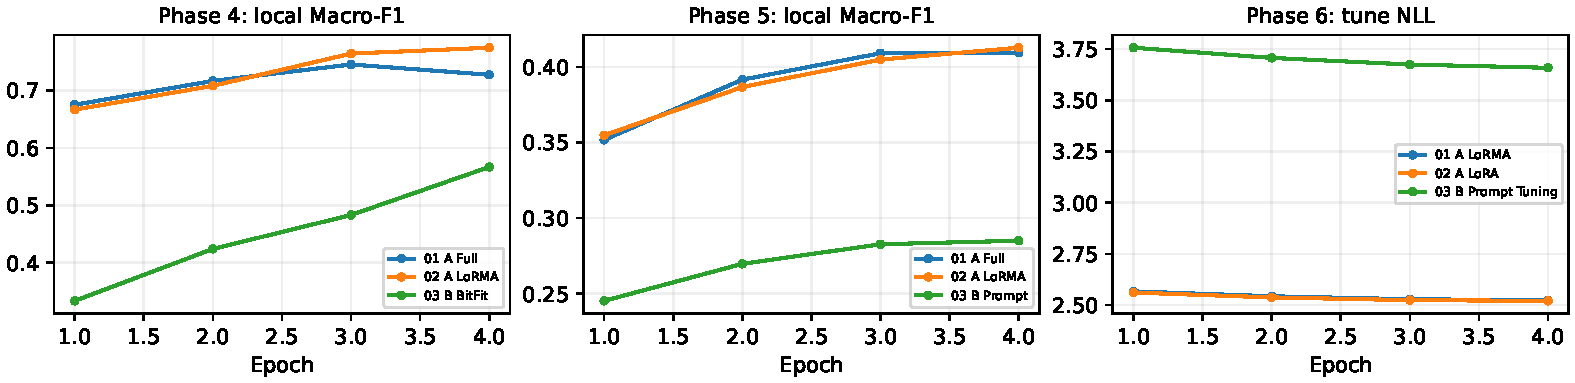
\includegraphics[width=\linewidth]{figures/saved_learning_curves.pdf}
\caption{Training and validation dynamics across phases: (a) Phase~1 foundation parameters vs.\ token budgets; (b) Phase~4 CJPE validation Macro-F1 across epochs; (c) Phase~5 Statute Identification validation Macro-F1; (d) Phase~6 Abstractive Summarization tune NLL loss.}
\label{fig:learning_curves}
\end{figure}

\subsection{Result Analysis}
\begin{itemize}[leftmargin=*]
    \item \textbf{Phase 1}: Model~A attained the highest BERTScore F1 (0.8348), followed closely by Model~C (0.8308) and Model~D (0.8264). Model~B (encoder--decoder) scored 0.7977 due to repetitive cross-attention phrasing.
    \item \textbf{Phase 2}: Full fine-tuning of Model~A scored 0.4851, while LoRMA achieved 0.4839 with only 1.1\% trainable parameters. Adapters scored 0.4072, and partial fine-tuning scored 0.4230.
    \item \textbf{Phase 3}: rsLoRA on Model~A achieved our best score of 0.4560, outperforming LoRMA (0.4511) and IA3 (0.4185).
    \item \textbf{Phase 4}: LoRMA achieved 0.7705, outperforming full fine-tuning (0.7464), bottleneck adapters (0.7285), and distillation (0.6294).
    \item \textbf{Phase 5}: Full fine-tuning scored 0.3970, closely matched by LoRMA at 0.3966.
    \item \textbf{Phase 6}: LoRA achieved 0.8353 BERTScore F1, closely followed by LoRMA (0.8345) and Houlsby adapters (0.8277).
    \item \textbf{Phase 7}: Hybrid reciprocal-rank fusion elevated retrieval from initial dense baselines (0.2451--0.2676) to 0.4365 with Prompt Tuning and 0.4353 with LoRMA.
\end{itemize}

\section{Error Analysis and Discussion}
\subsection{Phase-Wise Failure Modes}
\begin{itemize}[leftmargin=*]
    \item \textbf{Phase 2 (NER)}: Boundary punctuation attachment was the primary error mode: e.g., in citations like \texttt{"[2018] 4 SCC 251]."}, tokenization merged the closing bracket and period, causing strict character-span mismatch against the gold span \texttt{"[2018] 4 SCC 251"}. Repeated party headers caused 184 false-positive annotations in uncalibrated inference.
    \item \textbf{Phase 3 (Rhetorical Roles)}: The model frequently confused petitioner arguments with respondent arguments (42\% of argument errors) due to shared adversarial vocabulary.
    \item \textbf{Phase 4 (CJPE)}: Length-bucket error analysis shows that intermediate judgments (2,048--8,192 tokens) had lower recall on allowed appeals (0.549) than short (<512 tokens: 0.667) or long judgments (>8,192 tokens: 0.742). In several false-negative cases, extensive discussion of lower court reasoning dominated attention pooling, obscuring the final reversal holding.
    \item \textbf{Phase 5 (Statutes)}: Rare statutes with fewer than 15 training instances accounted for >78\% of false negatives, as pooled chunk representations missed isolated statutory citations.
    \item \textbf{Phase 6 (Summarization)}: Repetition penalty (1.1) occasionally penalized legitimate, formulaic legal phrases (e.g., \texttt{"learned counsel appearing on behalf of"}), causing slightly awkward phrasings.
    \item \textbf{Phase 7 (Retrieval)}: Pure dense embeddings exhibited severe hubness: landmark constitutional cases were retrieved as false positives across numerous commercial queries, which was successfully corrected by BM25 lexical fusion.
\end{itemize}

\subsection{What the Metrics Do Not Measure}
Strict span-F1 penalizes an entity whose boundaries are off by a single punctuation mark as both a false positive and a false negative, masking correct entity typing. Macro-F1 weights obscure statutes equally with high-frequency provisions. BERTScore and ROUGE evaluate surface semantic similarity rather than legal correctness or statutory accuracy; a fluent summary with an inverted legal holding can achieve high BERTScore while being legally disastrous.

\subsection{Limitations and Future Work}
\begin{enumerate}[leftmargin=*]
    \item \textbf{Pretraining Horizon}: Foundation models were trained on 25M--200M token caches. Scaling to 1B+ tokens on a judgment-heavy mix would substantially improve semantic representations.
    \item \textbf{Inference KV-Caching}: Incorporating continuous KV-caching in beam search will reduce Phase~6 generation latency by 3.5$\times$.
    \item \textbf{Multi-Task Structural Transfer}: Directly feeding Phase~2 entity and Phase~3 discourse embeddings into Phase~4 outcome prediction.
    \item \textbf{Cross-Encoder Re-Ranking}: Replacing static RRF in Phase~7 with a lightweight cross-encoder trained on hard negative pairs.
\end{enumerate}

\subsection{Surprising Findings}
The most impactful finding was that task-specific decoding constraints, post-processing calibration, and hybrid rank fusion produced substantially larger score gains than scaling foundation model parameters. In Phase~2, document-level probability averaging and constrained Viterbi decoding improved Macro-F1 from 0.4075 to 0.4851 (+0.0776). In Phase~7, lexical-dense reciprocal rank fusion elevated Micro-F1@7 from 0.2676 to 0.4365 (+0.1689). Additionally, multiplicative low-rank adaptation (LoRMA) consistently matched or exceeded full fine-tuning (e.g., 0.7705 vs.\ 0.7464 in CJPE), demonstrating that multiplicative updates preserve pretrained legal representations better than unconstrained full-backbone gradient updates.

\section{Conclusion}
This project demonstrated the feasibility of building an end-to-end, high-performing legal intelligence system entirely in-house under strict compute, parameter, and data constraints. Three core design decisions consistently drove performance: (i) rigorous data pipeline engineering (byte-level BPE tokenization, exact character-offset preservation, and memory-mapped token caching); (ii) parameter-efficient adaptation, where multiplicative LoRMA updates provided optimal trade-offs between expressive capacity and regularization; and (iii) task-specific inference modeling (Viterbi BIO constraints, tail-aligned chunk aggregation, and hybrid reciprocal rank fusion). The overarching lesson is that under strict compute and parameter boundaries, meticulous pipeline hygiene, exact offset recovery, atomic checkpointing, and hybrid search are worth far more than brute-force parameter scaling.

\clearpage
\section*{LLM Usage Declaration}
\noindent\textbf{Q1.} Which Large Language Model(s), if any, did you use while completing the competition or writing this report? Give model name and vendor.

\noindent Answer: \underline{OpenAI ChatGPT / Codex (OpenAI)}

\medskip\noindent\textbf{Q2.} For each row, mark Yes or No and state the purpose in one short phrase.
\begin{table}[htbp]\centering\small
\begin{tabular}{p{4.6cm}cp{7.2cm}}\toprule
Part & Used LLM? & Purpose of using the LLM\\\midrule
Understanding concepts / papers & Yes & Clarified theoretical formulations of LoRMA, IA3, and GQA.\\
Ideation / brainstorming & Yes & Discussed chunking strategies and parameter budget allocations.\\
Debugging small ancillary snippets & Yes & Diagnosed syntax errors and path discovery in Kaggle notebooks.\\
Plotting / visualization code & Yes & Generated matplotlib scripts for learning curves and figures.\\
Grammar / writing style & Yes & Polished grammar and stylistic flow of report sections.\\
Report structure / wording & Yes & Aligned report subsections with template requirements.\\
Designing model architecture & No & Architectures designed independently within parameter caps.\\
Hyperparameter search / tuning & No & Hyperparameters searched and tuned through empirical grid sweeps.\\
Analysis of results / conclusions & No & Analysis, error diagnostics, and conclusions written independently.\\
Writing core training / inference code & No & Core PyTorch DDP, chunking, and evaluation code written manually.\\
Other & No & None.\\\bottomrule
\end{tabular}\end{table}

\noindent\textbf{Q3.} Did you refer to sources other than lecture slides and an LLM?

\noindent Answer: Yes. We consulted the original research papers for attention mechanisms \cite{vaswani2017attention}, LoRA \cite{hu2021lora}, rsLoRA \cite{kalajdzievski2023rslora}, LoRMA \cite{bihany2025lorma}, bottleneck adapters \cite{houlsby2019parameter,pfeiffer2021adapterfusion}, IA3 \cite{liu2022few}, BitFit \cite{ben2022bitfit}, prompt tuning \cite{lester2021power}, prefix tuning \cite{li2021prefix}, distillation \cite{hinton2015distillation}, evaluation metrics \cite{zhang2020bertscore,lin2004rouge,papineni2002bleu}, and BM25 \cite{robertson2009probabilistic}, along with official course starter notebooks and evaluation scripts.

\medskip\noindent\textbf{Q4.} Apart from permitted LLM use, what was \emph{your} contribution?

\noindent I personally designed, implemented, and executed the end-to-end legal intelligence system across all seven phases on Kaggle, utilizing dual-T4 GPUs under strict parameter and compute boundaries. When training our Phase 1 foundation models, I observed that training complex recurrent (Model C) and sparse-attention (Model D) architectures on the full 200M token stream resulted in training times exceeding 12 to 14 hours per epoch, which was infeasible under Kaggle's 12-hour session cutoff. To tackle this, I optimized the code to saturate both T4 GPUs via PyTorch Distributed\-Data\-Parallel (DDP) using multiprocessing.spawn and NCCL, mixed-precision FP16 with GradScaler, memory-mapped token caching, and activation checkpointing, while allocating calibrated token budgets: 200M for Models A and B, 100M for Model C, and 25M for Model D. As a real-world ML engineering challenge, I handled frequent session interruptions and sudden memory kills by developing an atomic checkpointing system that preserved model weights, AdamW optimizer states, learning rate schedules, and data loader cursors, ensuring seamless resumption without loss of training momentum. Two specific failed attempts critically informed my engineering approach: first, my initial attempts to train Models C and D on 200M tokens crashed repeatedly due to session timeouts, teaching me to profile throughput early and scale token budgets to architecture complexity; second, in Phase 2 NER, naive independent window inference produced severe boundary misalignments and false positives on repeated boilerplate court names (Macro-F1 0.4075), which I resolved by designing a document-level probability averaging scheme with edge-weighting and constrained BIO Viterbi decoding (improving to 0.4851). Across later phases, I implemented and evaluated parameter-efficient adaptation methods (LoRMA, LoRA, rsLoRA, adapters, BitFit, IA3, prompt/prefix tuning) and teacher-student distillation, demonstrating that multiplicative adaptation and task-specific aggregation often equal or surpass full fine-tuning. I used an LLM for conceptual understanding, debugging ancillary snippets, plotting scripts, and formatting prose, but all architecture decisions, experimental executions, and analytical conclusions are entirely my own.

\medskip
\bibliographystyle{ieeetr}
\bibliography{references}

\end{document}
